% !TeX root = ../main.tex
% Add the above to each chapter to make compiling the PDF easier in some editors.

\chapter{Algorithms for Maximum Flow}

In this chapter, we study classical combinatorial algorithms for the maximum flow problem. Many of the algorithms can be adapted to solve the more general minimum-cost flow problem. In recent years, we have made significant progress by using convex optimization and interior point methods.

We consider directed graphs $G = (V, E, \vc)$ with edge capacities $\vc \in \R^{|\sE|}$. Recall that a \emph{flow}\index{flow} is a vector $\vf \in \R^{|\sE|}$ and $\vf$ routes demands $\vd$ iff $\mB\vf = \vd$. We say that $\vf$ is \emph{feasible}\index{feasible flow} iff $\vZero \leq \vf \leq \vc$, where $\vZero \leq \vf$ ensures that the flow respects edge directions and $\vf \leq \vc$ ensures that the flow respects edge capacities.

We call a flow $\vf$ that routes demands $F(\vOne_t - \vOne_s)$ for some $F \in \R$ and vertices $s,t \in \sV$, so $F$ units of flow from $s$ to $t$, an \emph{$s$-$t$ flow}\index{s-t flow} with \emph{value}\index{flow value} $\val(\vf) = F$. We say that $\vf$ is \emph{optimal} iff there is no feasible $s$-$t$ flow $\vf'$ such that $\val(\vf') > \val(\vf)$.

We can decompose any $s$-$t$ flow into two kinds of flows: path flows and cycle flows.

\begin{defn}[Path flow]
An \emph{$s$-$t$ path flow}\index{$s$-$t$ path flow} $\vf$ is an $s$-$t$ flow with $\val(\vf) = \alpha$ for some $\alpha > 0$ that can be expressed as, \begin{align}
    \vf = \alpha\sum_{e \in \sP} \vOne_e,
\end{align} for some $s$-$t$ path $\sP$.
\end{defn}
\begin{marginfigure}
TBD
% \centering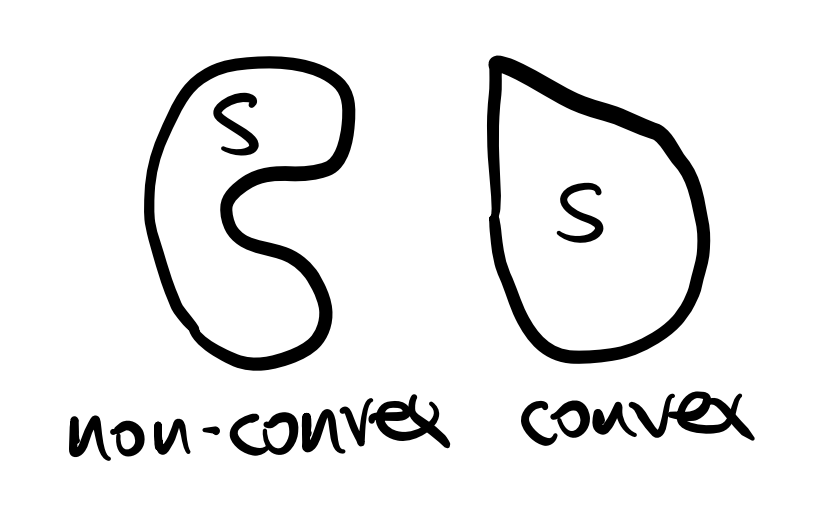
\includegraphics[width=4cm]{notes/figures/convex_set.png}
\caption{Example of an $s$-$t$ path flow.}
\end{marginfigure}
\begin{defn}[Cycle flow]
A \emph{cycle flow}\index{cycle flow} $\vf$ is a flow routing demands $\vZero$ that can be expressed as, \begin{align}
    \vf = \alpha\sum_{e\in\sC} \vOne_e,
\end{align} for some $\alpha > 0$, and cycle $\sC$.
\end{defn}
\begin{marginfigure}
TBD
% \centering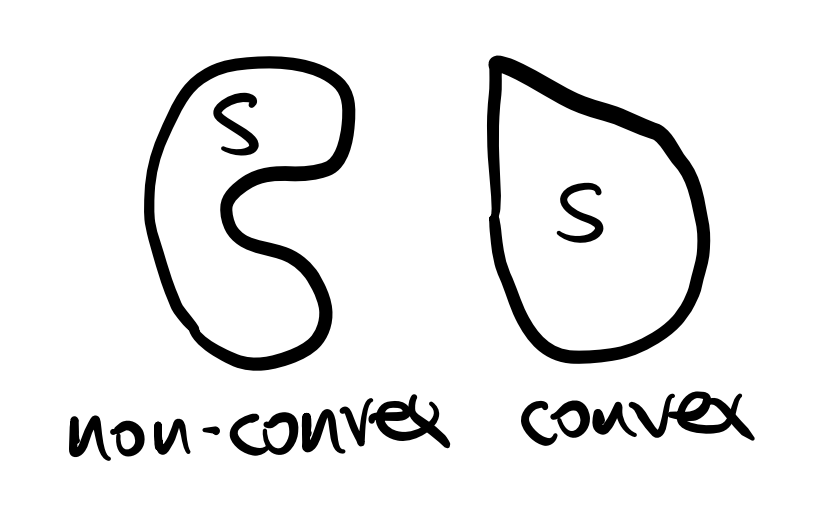
\includegraphics[width=4cm]{notes/figures/convex_set.png}
\caption{Example of a cycle flow.}
\end{marginfigure}
\begin{lem}[Path-cycle decomposition]
Any $s$-$t$ flow $\vf \geq \vZero$ can be decomposed into $k \leq m$ $s$-$t$ path flows and $l$ cycle flows.
\end{lem}
\begin{proof}
TBD
\end{proof}

\begin{lem}
There exists an optimal flow with a path-cycle decomposition that has only paths and no cycles.
\end{lem}
\begin{proof}
TBD
\end{proof}

\begin{lem}
There exists an $s$-$t$ flow $\vf \geq \vZero$ iff there exists a directed $s$-$t$ path.
\end{lem}
\begin{proof}
TBD
\end{proof}

Recall that a \emph{cut}\index{cut} is a proper subset of vertices $\emptyset \subset \sS \subset \sV$. An \emph{$s$-$t$ cut}\index{s-t cut} is a cut $(\sS, \sV \setminus \sS)$ separating $s$ and $t$, i.e., $s \in \sS, t \in \sV \setminus \sS$. We say that the capacity of a cut is the sum of capacities of crossing edges, \begin{align}
    \capa(\sS) \defeq \sum_{\substack{\{a,b\} \in \sE \\ a \in \sS,\ b \in \sV \setminus \sS}} \vc(\{a,b\}).
\end{align}

\begin{thm}[Weak duality of maximum flow/minimum cut]
For any feasible $s$-$t$ flow $\vf$ and any $s$-$t$ cut $(\sS, \sV \setminus \sS)$, \begin{align}
    \val(\vf) \leq \capa(\sS).
\end{align}
\end{thm}
\begin{proof}
Let $(\sS, \sV \setminus \sS)$ be any $s$-$t$ cut. Suppose for a contradiction that $\val(\vf) > \capa(\sS)$ for some flow $\vf$. But this contradicts feasibility of $\vf$ because the crossing edges of the cut form a bottleneck.
\end{proof}

An important concept in the analysis of flow algorithms is the so-called residual graph.

\begin{defn}[Residual graph]
The \emph{residual graph}\index{residual graph} $G_\vf$ of some $s$-$t$ flow $\vf \geq \vZero$ is the graph $G$ with edge capacities $[-\vf, \vc - \vf]$. That is, we say that a flow $\hat{\vf}$ is \emph{feasible} in the residual graph iff $-\vf \leq \hat{\vf} \leq \vc - \vf$.
\end{defn}

Intuitively, sending positive flow $\vc - \vf$ along an edge in $G_\vf$ corresponds to sending the maximum additional flow without violating the capacity constraint within $G$, whereas sending negative flow $-\vf$ along an edge in $G_\vf$ corresponds to ``undoing'' the flow that was send along this edge by $\vf$. This simple argument shows that if $\hat{\vf}$ is feasible in $G_\vf$, then $\vf + \hat{\vf}$ is feasible in $G$.

We call an $s$-$t$ flow $\hat{\vf}$ in $G_\vf$ an \emph{augmenting flow}\index{augmenting flow} of $\vf$.

\begin{lem}[Flow optimality condition]
A feasible $s$-$t$ flow $\vf$ in $G$ is optimal iff there is no $s$-$t$ path in $G_\vf$, or equivalently, iff there is no $\vf$-augmenting flow.
\end{lem}
\begin{proof}
TBD
\end{proof}

\begin{thm}[Strong duality of maximum flow/minimum cut]
We have that, \begin{align}
    \max_{\substack{F \in \R,\ \vf \in \R^{|\sE|} \\ \mB\vf = F(\vOne_t - \vOne_s)}} F = \min_{\text{$s$-$t$ cut $(\sS, \sV \setminus \sS)$}} \capa(\sS).
\end{align}
\end{thm}
\begin{proof}
By weak duality of maximum flow and minimum cut, we have the direction $\leq$. For the direction $\geq$, let $\s{\vf}$ be an optimal flow and consider the cut, \begin{align*}
    \sS \defeq \{v \in \sV \mid \text{there exists an $s$-$v$ path in $G_{\s{\vf}}$}\}.
\end{align*} We make two observations. \begin{enumerate}
    \item By definition, there are no edges from $\sS$ to $\sV \setminus \sS$ in $G_{\s{\vf}}$, that is, $\s{\vf}$ \emph{saturates}\footnote{That is, $\s{\vf}$ sends flow equal to the capacity of the edge.} all crossing edges of the cut.
    \item By definition, $\s{\vf}$ routes no flow from $\sV \setminus \sS$ to $\sS$.
\end{enumerate}\noindent This implies that $\val(\s{\vf}) \geq \capa(\sS)$ for this cut $(\sS, \sV \setminus \sS)$.
\end{proof}

\section{The Ford-Fulkerson Algorithm}

Our prior discussion gives rise to a very natural algorithm.

\begin{algorithm}
    \caption{\textsc{FordFulkerson($G$)}}\index{Ford-Fulkerson algorithm}
    $\vf \gets \vZero$\;
    \While{there exists any $s$-$t$ path flow $\hat{f}$ in $G_\vf$}{
        $\vf \gets \vf + \hat{\vf}$\;
    }
    \Return{$\vf$}
\end{algorithm}

Given a feasible flow $\vf$, we can find an $\vf$-augmenting flow, or determine that none exists, in time $\LandauO{m}$ using breadth-first search or depth-first search.

\begin{thm}[Ford-Fulkerson]
If capacities are integral, \textsc{FordFulkerson} converges to an optimal flow $\s{\vf}$ in $\val(\s{\vf})$ iterations.
\end{thm}
\begin{proof}
Observe that the initial flow $\vZero$ is trivially feasible. In each iteration, we add the augmenting flow $\hat{\vf}$ with $\val(\hat{\vf}) > 0$, and due to the integral capacities, $\val(\hat{\vf}) \geq 1$. Therefore, the flow value $\val(\vf)$ increases in each iteration by at least one.
\end{proof}

\subsection{Improving Ford-Fulkerson}

It turns out that if we always choose the shortest augmenting path, we converge in time $\LandauO{n m^2}$. This is known as the \emph{Edmonds-Karp algorithm}\index{Edmonds-Karp algorithm}.

We can do still better, by choosing that path with the maximum bottleneck capacity. That is, we choose, \begin{align}
    \s{\sP} = \argmax_{\text{augmenting paths $\sP$}} \min_{e \in \sP} \vc(e).
\end{align} Within the framework of Ford-Fulkerson this corresponds to the augmenting path that allows us to route the most additional flow.

\begin{thm}
\textsc{FordFulkerson}, where in each iteration we choose the augmenting path with maximum bottleneck capacity, converges in time $\LandauO{m^2 \log mU}$.
\end{thm}
\begin{proof}
We can find $\s{\sP}$ using a binary search on $[1,U]$, where $U \defeq \max_e \vc(e)$, by removing all edges with absolute capacity in $G_\vf$ below the current threshold and testing if an $s$-$t$ path in $G_\vf$ exists: if it does, we increase the threshold; if it does not, we decrease the threshold. This procedure takes $\LandauO{m \log U}$ time. If we only consider the occurring capacities, the runtime improves to $\LandauO{m \log m}$.

Suppose $\hat{F}$ is the flow left in $G_\vf$. By the path decomposition lemma, this flow can be decomposed into at most $m$ path flows (the ``best'' of which is $\s{\sP}$) and $\s{\sP}$ must route at least the average amount of flow. Hence, $\s{\sP}$ routes at least $\nicefrac{\hat{F}}{m}$ units of flow. Thus, the algorithm converged if, \begin{align*}
    \parentheses*{1 - \frac{1}{m}}^T \s{F} < 1,
\end{align*} where $T$ is the number of augmentations and $\s{F}$ is the value of an optimal flow. So, some $T = \LandauO{m \log \s{F}}$ is sufficient.

Overall, we get, \begin{align*}
    \LandauO{m \log m \cdot T} = \LandauO{m^2 \log (m+\s{F})} = \LandauO{m^2 \log mU} \margintag{using $\s{F} \leq mU$} &\qedhere
\end{align*}
\end{proof}

\section{Dinitz's Algorithm}
\section{The Push-Relabel Algorithm}
\section{Outlook}